\section{Resultados}

El primer experimento se realiz\'0 utilizando una lista de 27 p\'aginas web, las cuales devolvieron un
total de 26 links (tan solo 10 de ellas dieron una cantidad positiva).

Aqu\'i la lista:\\
www.google.com\\ 
www.clarin.com\\
www.clarin.com/deportes\\
www.lanacion.com.ar/\\    
www.infobae.com\\
canchallena.lanacion.com.ar\\
www.rollingstone.com.ar\\
www.ole.com.ar\\
www.clasificados.clarin.com\\
www.mamapuntocero.com.ar\\
www.ciudad.com.ar\\
www.zonaprop.com.ar\\
www.pagina12.com.ar\\
www.yahoo.com\\
www.taringa.net\\
www.mercadolibre.com.ar\\
www.youtube.com\\
www.netbeans.com\\
www.github.com\\
www.assembla.com\\
www.gmail.com\\
www.hotmail.com\\
www.facebook.com\\
www.twitter.com\\
maps.google.com.ar\\
www.stackoverflow.com\\
www.9gag.com\\

\subsection{Propagaci\'on del error}

El experimento fue realizado variando la constante c, la cual determina la importancia proporcional que se quiere
entre la probabilidad de pasar a una p\'agina desde un link (c mas alto) contra la de escribir la url a mano (c mas bajo).

El criterio de parada es la diferencia de norma uno entre el autovector que se obtiene
en cada iteraci\'on y el de la iteraci\'on anterior, el cual no debe ser menor que un
epsilon de orden -15.

\begin{figure}[H]
  \centering
    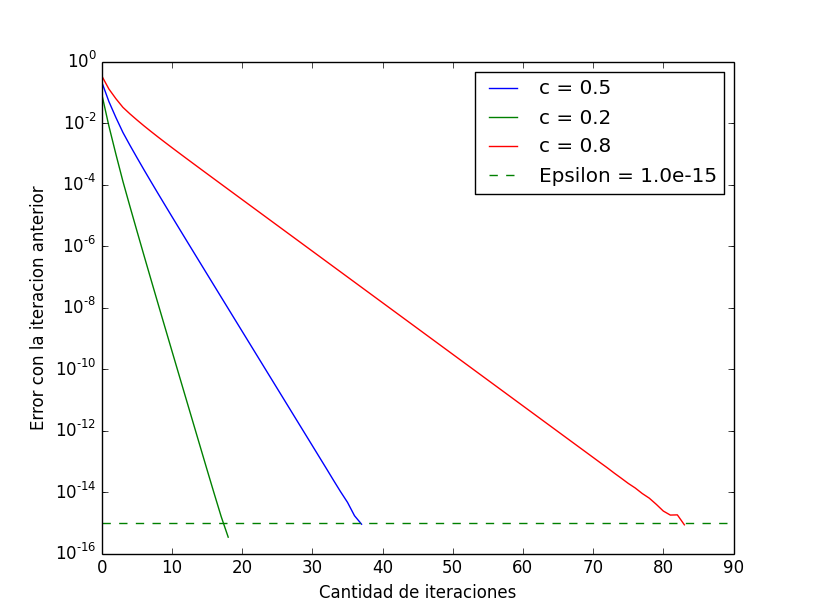
\includegraphics[width=0.9\textwidth]{../parser/graficoError1.png}
    \caption{}
    \label{}
\end{figure}

Se puede obvservar en la figura que cuanto menor es el c, m\'as r\'apido converge
el m\'etodo. Creemos que dicho resultado se debe a que al darle menor importancia
a los links directos, la matriz de probabilidades se encuentra mejor balanceada, 
por lo tanto los primeros autovalores de ella son mas parecidos y por ello se necesitan
m\'as iteraciones para lograr la convergencia. De hecho, se prob\'o bajar mas el epsilon,
el resultado fue que cuando c = 0.8 el m\'etodo no converge, mientras que para c = 0.2 y
c = 0.5 el m\'etodo se estabiliza en pocos pasos m\'as de los que muestra el gr\'afico, dejando
un error igual a 0.




